\section{A Taxonomy of Explanation Methods}
\label{sec:taxonomy}

Fig.~\ref{fig:taxonomy} organises the methods along two axes: how the explanation is produced and what it refers to. Table~\ref{tab:taxonomy} places the reviewed studies in it. Of the 41 appraised studies, 24 rely on post-hoc methods, 11 are intrinsic, five combine the two, and one claims interpretability without showing any explanation.

\begin{figure*}[!t]
\centering
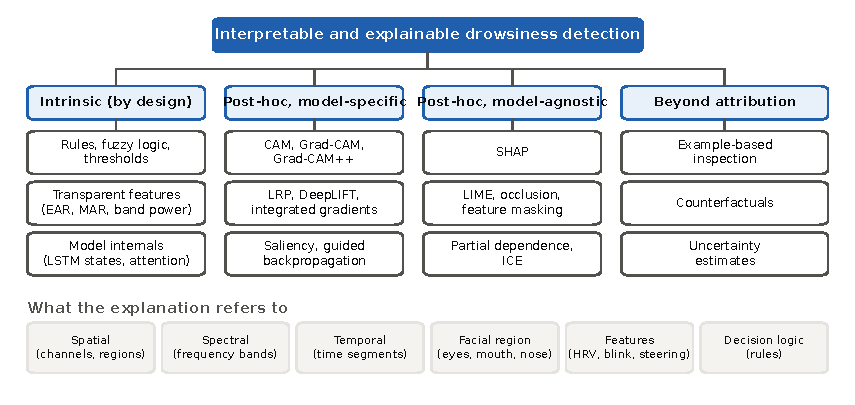
\includegraphics[width=\textwidth]{fig1_taxonomy}
\caption{Taxonomy used in this review. The upper part groups methods by how the explanation is produced; the lower band lists what an explanation can refer to. EAR: eye aspect ratio; MAR: mouth aspect ratio; ICE: individual conditional expectation.}
\label{fig:taxonomy}
\end{figure*}

\subsection{Intrinsic methods}
\textit{Rules and logic.} Rule-based systems make every decision traceable. Beles \textit{et al.}~\cite{beles2024driver} fuse physiological and camera cues with fuzzy rules, and Ersoy \textit{et al.}~\cite{ersoy2026improving} calibrate eye and mouth thresholds to each driver. Fuzzy systems range widely in how readable they are. Gao \textit{et al.}~\cite{gao2025comprehensive} stack Takagi--Sugeno--Kang classifiers whose rules use linguistic levels but refer to features only by index, whereas Hu \textit{et al.}~\cite{hu2026human} and Yan and Xie~\cite{yan2026toward} write interval type-2 rules over named eye and mouth measures, the latter constraining the membership functions so that the sets stay ordered and distinguishable. Georgiadis \textit{et al.}~\cite{georgiadis2026timeaware} go furthest towards symbolic reasoning, with an ontology whose logic rules map physiological thresholds to driver states.

\textit{Transparent features.} Albadawi \textit{et al.}~\cite{albadawi2023realtime} feed eye aspect ratio, mouth aspect ratio and head position to simple classifiers, so an alarm can be traced to a named cue.

\textit{Model internals.} Other studies read explanations from LSTM hidden states \cite{cui2021subject}, attention scores \cite{an2024attention,gao2024sftnet} or the eigenvalues of a recurrent weight matrix \cite{gao2025idsrn}. Internal states are built in, but that does not establish that they explain the decision. Attention weights in particular need not track input importance \cite{jain2019attention}, and Section~\ref{sec:attention} shows that the question is live in this domain.

\subsection{Post-hoc, model-specific methods}
Class activation mapping (CAM) \cite{zhou2016cam} weights the last convolutional feature maps by the class weights of a global-average-pooling network. Grad-CAM \cite{selvaraju2017gradcam} extends the idea to other architectures using gradients, Grad-CAM++ \cite{chattopadhay2018gradcampp} uses higher-order gradient terms, and LayerCAM \cite{jiang2021layercam} weights each location by its positive gradients and works at any layer. This family dominates the vision studies. Layer-wise relevance propagation (LRP) \cite{bach2015lrp} passes the output score backwards layer by layer, and integrated gradients \cite{sundararajan2017axiomatic} accumulate gradients along a path from a baseline to the input. These produce finer-grained maps, and the integrated-gradients result depends on the chosen baseline. Attention rollout \cite{abnar2020quantifying} combines attention across transformer layers and needs the same testing as other attention maps; one reviewed study applies it across modalities \cite{theivadas2025dynamic}.

\subsection{Post-hoc, model-agnostic methods}
SHAP \cite{lundberg2017shap} assigns each feature a Shapley value and, in the studies reviewed, is applied mostly to tree models on hand-crafted features. LIME \cite{ribeiro2016lime} fits a simple local surrogate, and occlusion \cite{zeiler2014visualizing} measures the score drop when part of the input is hidden. PGM-Explainer perturbs graph nodes and fits a Bayesian network over them; it appears here in one study on a graph network \cite{zeynalpour2025multimethod}. Partial dependence \cite{friedman2001greedy} and individual conditional expectation plots \cite{goldstein2015ice} show how predictions change with a feature, but they assume the feature varies independently of the others, which is doubtful for correlated physiological measures.

\subsection{Beyond attribution}
Three other forms appear rarely. McDonald \textit{et al.}~\cite{mcdonald2014steering} explain a model by inspecting example inputs from each cell of the confusion matrix. Counterfactual explanations \cite{wachter2017counterfactual}, the smallest change that would flip a decision, have been proposed for drowsiness alarms \cite{jha2025realtime} but not evaluated. Uncertainty estimates \cite{oise2026enhancing} complement an explanation but do not attribute a decision.

\begin{table}[!t]
\centering
\caption{Placement of the Reviewed Studies in the Taxonomy}
\label{tab:taxonomy}
\footnotesize
\begin{tabularx}{\columnwidth}{@{}L{0.33\columnwidth}Y@{}}
\toprule
\textbf{Method family} & \textbf{Studies} \\
\midrule
\multicolumn{2}{@{}l}{\textit{Intrinsic}} \\
Rules, fuzzy logic & \cite{beles2024driver,ersoy2026improving,gao2025comprehensive,hu2026human,yan2026toward} \\
Ontology, logic rules & \cite{georgiadis2026timeaware} \\
Transparent features & \cite{albadawi2023realtime} \\
Model internals & \cite{cui2021subject,an2024attention,gao2025idsrn,gao2024sftnet} \\
\midrule
\multicolumn{2}{@{}l}{\textit{Post-hoc, model-specific}} \\
CAM family & \cite{cui2022eeg,cui2022compact,feng2025id3rsnet,wu2024driver,saxena2026lowlight,rafy2026domain,oise2026enhancing,nomura2025drowsiness,florez2023cnn,hassan2025realtime,zeynalpour2025multimethod,jewel2025lightweight,sasikala2026robust,nayomi2026vision} \\
LRP, integrated gradients & \cite{seo2025driver,saxena2026lowlight} \\
Feature-map visualisation & \cite{xu2026dynamic} \\
\midrule
\multicolumn{2}{@{}l}{\textit{Post-hoc, model-agnostic}} \\
SHAP & \cite{hasan2024validation,vitorino2023adversarial,puspasari2026predicting,zhou2021predicting,jha2025realtime,zhu2025madfm,guan2025fatigue,zeynalpour2025multimethod} \\
LIME, occlusion & \cite{saxena2026lowlight,zeynalpour2025multimethod} \\
PGM-Explainer & \cite{zeynalpour2025multimethod} \\
Partial dependence, ICE & \cite{hasan2024validation} \\
\midrule
\multicolumn{2}{@{}l}{\textit{Combined}} \\
Selection pipeline + SHAP & \cite{jiang2026eeg} \\
Kernel weights + masking & \cite{zhou2026sedriven} \\
Rule + Grad-CAM & \cite{florez2024realtime} \\
Graph attention + occlusion & \cite{zhuang2024connectivity} \\
Modality attention + saliency & \cite{theivadas2025dynamic} \\
\midrule
\multicolumn{2}{@{}l}{\textit{Other}} \\
Example inspection & \cite{mcdonald2014steering} \\
Band correlation, t-SNE & \cite{zhang2024multimodal} \\
Counterfactuals & \cite{jha2025realtime} \\
Uncertainty & \cite{oise2026enhancing} \\
Claimed, none shown & \cite{alarnaout2025exploiting} \\
\bottomrule
\end{tabularx}
\end{table}
